% \iffalse meta-comment
%
% Copyright (C) 2015 by Henrik Skov Midtiby <henrikmidtiby@gmail.com>
% -------------------------------------------------------
% 
% This file may be distributed and/or modified under the
% conditions of the LaTeX Project Public License, either version 1.2
% of this license or (at your option) any later version.
% The latest version of this license is in:
%
%    http://www.latex-project.org/lppl.txt
%
% and version 1.2 or later is part of all distributions of LaTeX 
% version 1999/12/01 or later.
%
% \fi
%
% \iffalse
%<*driver>
\ProvidesFile{todonotes.dtx}
%</driver>
%<package>\NeedsTeXFormat{LaTeX2e}[1999/12/01]
%<package>\ProvidesPackage{todonotes}
%<*package>
    [2018/10/17 v1.1 Todonotes source and documentation.]
%</package>
%
%<*driver>
\documentclass{ltxdoc}
\usepackage{wrapfig}
\usepackage[colorlinks, linkcolor=black, urlcolor=blue]{hyperref}
\usepackage[colorinlistoftodos, shadow]{todonotes}[2018/10/17]
\usepackage{amsmath}
\usepackage{setspace}
\usepackage{soul}
\setcounter{tocdepth}{2}
\EnableCrossrefs         
\CodelineIndex
\RecordChanges
\begin{document}
  \DocInput{todonotes.dtx}
%\iffalse
%  \PrintChanges
%  \PrintIndex
%\fi
\end{document}
%</driver>
% \fi
%
% \CheckSum{696}
%
% \CharacterTable
%  {Upper-case    \A\B\C\D\E\F\G\H\I\J\K\L\M\N\O\P\Q\R\S\T\U\V\W\X\Y\Z
%   Lower-case    \a\b\c\d\e\f\g\h\i\j\k\l\m\n\o\p\q\r\s\t\u\v\w\x\y\z
%   Digits        \0\1\2\3\4\5\6\7\8\9
%   Exclamation   \!     Double quote  \"     Hash (number) \#
%   Dollar        \$     Percent       \%     Ampersand     \&
%   Acute accent  \'     Left paren    \(     Right paren   \)
%   Asterisk      \*     Plus          \+     Comma         \,
%   Minus         \-     Point         \.     Solidus       \/
%   Colon         \:     Semicolon     \;     Less than     \<
%   Equals        \=     Greater than  \>     Question mark \?
%   Commercial at \@     Left bracket  \[     Backslash     \\
%   Right bracket \]     Circumflex    \^     Underscore    \_
%   Grave accent  \`     Left brace    \{     Vertical bar  \|
%   Right brace   \}     Tilde         \~}
%
%
% \changes{0.1}{2008/04/17}{The first version of the package}
% \changes{0.2}{2008/05/15}{Updated the option handling of the package}
% \changes{0.2.1}{2008/05/16}{Slightly modified by Kjell Magne Fauske to 
%             support notes in the left margin (for documentstyle book).}
% \changes{0.2.2}{2008/05/28}{Added a missingfigure command}
% \changes{0.2.3}{2008/06/10}{Made a dependency on the calc package}
% \changes{0.3}{2008/07/11}{Delayed the requirements for the hyperref package
%             untill begin document and added an optional argument
%             to the todo command for adding inline todonotes (Idea
%             from Patrick Toche)}
% \changes{0.3.1}{2008/07/15}{Added some options to the todo macro (Idea: Patrick
%             Toche) and made the \\listoftodos point at the inserted
%             todos and not only the current / previous section, 
%             subsection or figure using the \\phantomsection macro.}
% \changes{0.4}{2008/07/28}{Modified the behaviour of the inline todonotes, to
%             avoid empty lines around the inline todonotes.}
% \changes{0.4.1}{2008/07/28}{
%             Added the option colorinlistoftodos which inserts a
%             small box with the used fillcolor of the todonotes in
%             the list of todos.}
% \changes{0.4.2}{2008/07/30}{Fixed a bug with the disable option to the
%             package.}
% \changes{0.5}{2008/08/05}{Created a dtx file containing both source
%             code and documentation of the package}
% \changes{0.5.1}{2008/09/15}{Updated the documentation}
% \changes{0.5.2}{2008/10/20}{Fixed a bug that prevented the usage
%             of the option french for babel. Bug report by Thomas
%             Braun.}
% \changes{0.6}{2008/10/24}{Added the caption option to the todo
%             command.}
% \changes{0.6.1}{2008/11/07}{Added a new usecase with decreased line
%             spacing.}
% \changes{0.6.2}{2008/11/13}{Added a usecase by Fabrice Niessen.}
% \changes{0.7}{2008/11/22}{Added language options on request from
%             Peter Zimmermann.}
% \changes{0.7.1}{2008/12/07}{Reworked the color options for both
%             the whole package and the todo command. General code
%             clean up. Added the prependcaption package option.}
% \changes{0.7.2}{2008/12/27}{Avoid to change the fontsize inside
%             the list of todos, fixing a bug revealed by Vladimir
%             Zhuravlev.}
% \changes{0.7.3}{2008/12/30}{The localization options (danish and
%             german) and the disable options, were all flawed by
%             naming inconsistencies that made then break the
%             package. This have been fixed.}
% \changes{0.7.4}{2008/12/30}{Fixed a bug related to the caption
%             option for the todo command. Introduced a counter of
%             the number of inserted todos.}
% \changes{0.7.5}{2009/01/02}{Fixed a typo in a macroname.}
% \changes{0.7.6}{2009/01/04}{Added a textsize option for the
%             package and the prepend / noprepend option for the
%             todo command.}
% \changes{0.8}{2009/01/09}{Added three new translations french,
%             spanish and catalan thanks to Richard Dominique and
%             Joan Queralt. Improved the visual appearence of the
%             inserted notes (rounded corners and optional shadows) 
%             with code from Joan Queralt. Found an untranslated
%             textstring ''Figure'' in the source. Added a figwidth
%             option to the missingfigure command, patch by Paul
%             Ivanov.}
% \changes{0.8.1}{2009/01/12}{Added a space between the colored
%             square and the text in the list of todos. Added a new
%             usecase for marking old / new sections. Made the name
%             of listoftodos changeable.}
% \changes{0.8.2}{2009/02/04}{Italian translation by Gustavo
%             Cevolani. Removed the dependence on the hyperref
%             package.}
% \changes{0.8.3}{2009/03/31}{Added a use case for linking to the 
%             list of todos, idea from Andreas Plank. Introduced a
%             package option for listening to the draft option given
%             to the document class.}
% \changes{0.8.4}{2009/04/02}{Fixed a bug related to the obeyDraft
%             option.} 
% \changes{0.8.5}{2009/08/01}{Added two new usecases (enumeration of 
%             inserted todonotes and how to set custom default values). 
%             Changed the order of the use case examples.}
% \changes{0.8.6}{2009/08/05}{Added a portuguese translation by Og DeSouza.}
% \changes{0.8.7}{2009/10/24}{Updated portuguese translation. Added a ngerman 
%             alias for the german translation suggested by Michael Niedermair.}
% \changes{0.8.8}{2009/12/07}{Added a new usecase from Vitaly. Fixed a 
%             bug reported by Oscar Gustafsson. Explained why the placement
%             of todonotes in the margin fails in certain custom document classes.}
% \changes{0.8.9}{2009/12/25}{Added a dutch translation by Ruben Ruben Vermeersch.}
% \changes{0.9.0}{2010/09/13}{Added a english option as suggested by Marco Berghoff.}
% \changes{0.9.1}{2010/09/13}{Added the todototoc command by idea from Sven Augustin.}
% \changes{0.9.2}{2010/09/13}{Use chapter (if available) for the list of todos heading.}
% \changes{0.9.3}{2010/09/13}{Make an internal definition of the todo command, 
%             for easing redefinition of the command behaviour.}
% \changes{0.9.4}{2010/09/26}{Make the disable option work on a local scale.}
% \changes{0.9.5}{2010/09/26}{Code simplification by extracting functionality to 
%             smaller macros.}
% \changes{0.9.6}{2010/11/04}{Give fontsize to TikZ. Align notes with line where note 
%             is set. Added new option fancyline. Patches by Benjamin Kellermann.}
% \changes{0.9.7}{2011/03/07}{Updated documentation.}
% \changes{0.9.8}{2011/04/21}{Suppress warnings about underfull / overful boxes 
%             generated by the inserted todonotes. Patch by Peter M Schuler.}
% \changes{0.9.9}{2011/10/22}{Added author option, implementation provided by 
%             Xavier Alameda-Pineda. Example of modifying the 
%             listoftodos removing some protect commands with no effect.}
% \changes{1.0.0}{2012/07/25}{Mention trouble with the classicthesis style. 
%             Refer to some alternatives to the package.
%             Added todoin command as suggested by Stefan Pinnow.
%             Described how to use tikz externalize with todonotes.
%             Added obeyDraft and obeyFinal options.}
% \changes{1.0.1}{2012/11/24}{Fix spacing issues reported by Jonathan Zachhuber and 
%             Brent Longborough.
%             Added figheight option to the missingfigure command as suggested by Kim Albertsson.}
% \changes{1.0.2}{2014/07/14}{Added Swedish translation by Emil Lundberg. 
%             Added usecase by Tobias Winchen.
%             Mentioned that default arguments can be set using the presetkeys command.
%             Updated list of alternatives to the todonotes package.
%             Draw borders around coloured boxes in the list of todos, patch by Ze Loff.}
% \changes{1.0.3}{2014/10/21}{Added the option figcolor to missing figure, patch by Pascal Hebbeker.
%             Added Croatian translation by Ican Kokan.
%             Changed default with of missingfigure.
%             Removed some underfull box warnings, solution by Ernst Blecha.} 
% \changes{1.0.4}{2015/07/09}{Restructured documentation and placed some examples in the 
%             doc/examples subdirectory.}
% \changes{1.0.5}{2016/11/02}{Example of how to change the space eating behaviour 
%             added by Anselm Wagner. 
%             Reduced the width of missingfigure to avoid bad box warnings.}
% \changes{1.0.6}{2018/07/09}{Changed how whitespaces are handled around inserted 
%             todos to better mimick macros like index (Suggestion by Frank Mittelbach). 
%             Fix missing character warnings using patch by Niels Anders Danielsson. 
%             Use the specified textsize for missingfigure, patch by Johannes Twittmann. 
%             Added new options for inline todonotes based on code from Daniel Krenn. 
%             Added warning message when marginparwidth is less than 2cm, as 
%             suggested by ErikBoesen.}
% \changes{1.0.7}{2018/07/09}{Changed the warning about marginparwidth to a 
%             proper warning message.} 
% \changes{1.0.8}{2018/09/08}{Improved spacing behaviour so it mimics the index macro, 
%             patch by Frank Mittelbach. 
%             Center graphics vertically in missingfigure, patch by Philipp Allgeuer.
%             Added new option tickmarkheight as suggested by Richard Niland.}
% \changes{1.1.0}{2018/10/17}{Many improvements to the user interface by Frank Mittelbach.
%             Added the command setuptodonotes. Added textcolor as an option.
%             Marked the insertion point of notes with tickmarks with a customizable height.
%             Steamline which options that are accepted to size commands 
%             (both commands (backslash tiny) and text (tiny) are now supported).} 
% \GetFileInfo{todonotes.dtx}   
%
% \DoNotIndex{\newcommand,\newenvironment}
%
% \iffalse
% A macro for marking things todo before the next relase
% (typically update of documentation).
% \fi
% \newcommand{\donow}[1]{\todo[color=blue]{#1}}
% 
%
% \title{The \textsf{todonotes} package\thanks{This document
%   corresponds to \textsf{todonotes}~\fileversion, dated \filedate.}}
% \author{Henrik Skov Midtiby \\ \texttt{henrikmidtiby@gmail.com}}
%
% \maketitle
%
% \begin{abstract}
% The |todonotes| package allows you to insert to--do items in your
% document. At any point in the document a list of all the inserted
% to--do items can be listed with the |\listoftodos| command.
% \end{abstract}
%
% \tableofcontents
%
% \newpage
% \section{Introduction}
%
% The |todonotes| package makes three commands available to the
% user: |\todo[]{}|, |\missingfigure{}| and |\listoftodos|.
% |\todo[]{}| and |\missingfigure{}| makes it possible to insert
% notes in your document about things that has to be done later
% (todonotes \ldots).
% I developed the basic functionality of the package while I worked
% on my bachelor project.
% 
% Some alternatives for the todonotes package are:
% \begin{itemize}
% \item \href{http://ctan.org/pkg/easy-todo}{easy-todo}\\
% Depends on |color|, |tocloft| and |ifthen|, small feature set.
% \item \href{http://ctan.org/pkg/fixmetodonotes}{fixmetodonotes}\\
% Depends on |graphicx|, |color|, |transparent|, |watermark|,|fix-cm|, |ulem| and |tocloft|, small feature set.
% \item \href{http://ctan.org/pkg/todo}{todo}\\
% Depends on |amssymb|, medium feature set.
% \item \href{http://ctan.org/pkg/fixme}{fixme}\\
% Large package with a lot of features.
% \end{itemize}
% The main reason for considering other packages is that the todonotes 
% package is quire large and relies heavily on tikz.
% This can slow down compilation of large documents significantly.
% The mentioned alternatives have a different feature set and does not 
% rely on tikz, which makes them require less ressoureces.
%
%
% \subsection{Usage}
%
% \DescribeMacro{\todo}
% My \index{\todo}most common usage of the todonotes package, is to 
% insert an todonotes somewhere in a latex document. 
% An example of this usage is the command 
%
% |\todo{Make a cake \ldots}|, 
% 
% \noindent
% which renders like\todo{Make a cake \ldots}.
% The |\todo| command has this structure: 
% |\todo|\oarg{options}\marg{todo text}.
% The |todo text| is the text that will be shown in the todonote and
% in the list of todos. The optional argument |options|, allows the
% user to customize the appearance of the inserted todonotes.
% For a description of all the options see section
% \ref{subsecTodoOptions}.
%
%
% \DescribeMacro{\missingfigure}
% The |\missingfigure| command inserts an image containing an 
% attention sign and the given text.
% The command takes only one argument
% |\missingfigure|\marg{text}, a text string that could
% describe what the figure should consist of.
% An example of its usage could be 
%
% |\missingfigure{Make a sketch of the structure of a trebuchet.}| 
%
% \noindent
% which renders like.
%
% \missingfigure{Make a sketch of the structure of a trebuchet.}
%
%
% \DescribeMacro{\listoftodos}
% The |\listoftodos| command inserts a list of all the todos in the
% current document. |\listoftodos| takes no arguments.
% For this document the list of to--do's looks like.
% \listoftodos
% \vspace{0.5cm}
%
% \DescribeMacro{\todototoc}
% The |\todototoc| command adds an entry to the table of contents for 
% list of todos. The command should be placed right before the 
% |\listoftodos| command.
%
% \subsection{Package options}
% \label{subsecPackageOptions}
% \DescribeMacro{disable}
% If the option |disable| is passed to the package, the macros
% usually defined by the package (|\todo|, |\listoftodos| and
% |\missingfigure|) are defined as macros with no effect, and thus
% all inserted notes are removed.
%
% \DescribeMacro{obeyDraft, obeyFinal}
% When the option |obeyDraft| is given, the package checks
% if the one of the options |draft|, |draftcls| or |draftclsnofoot| 
% is given (this option is usually given to
% the documentclass). If the |draft| option is given, the
% functionality of the package is enabled and otherwise the effect
% of the package is disabled.
% The option |obeyFinal| does something similar, except that the 
% todonotes package is only disabled if the |final| option given.
%
% \DescribeMacro{danish, german, ngerman, english, french, swedish}
% \DescribeMacro{spanish, catalan, italian}
% \DescribeMacro{portuguese, dutch, croatian}
% Use translations of the text strings 
% ''List of todos'' and ''Missing figure''.
% The default is to use none of these options, which results in
% english text strings.
% Currently the following languages are supported: 
% catalan,
% croatian,
% danish,
% dutch,
% english, 
% french,
% german,
% ngerman,
% italian,
% portuguese,
% spanish and
% swedish.
% 
% \DescribeMacro{colorinlistoftodos}
% Adds a small colored square in front of all items in the Todo
% list. The color of the square is the same as the fill color of the
% inserted todonote.
% This can be useful if there are different types of todos 
% (insert reference, explain in detail, \ldots) where the color of
% the inserted todonote marks the type of todo.
%
% \DescribeMacro{color}
% \DescribeMacro{backgroundcolor}
% \DescribeMacro{textcolor}
% \DescribeMacro{linecolor}
% \DescribeMacro{bordercolor}
% These options sets the default colors for the todo command.
% There are four colors that can be specified. The border color
% (default |bordercolor=black|) around the inserted text, the color
% behind the inserted text (default |backgroundcolor=orange|), the 
% color of the inserted text (default |textcolor=black|) and
% the color of the line connecting the inserted textbox with the
% current location in the text (default |linecolor=orange|). 
% Setting the |color| option to |val| passes this value on to the 
% background and line color options.
% The specified colors must be valid according to the 
% |xcolor| package.
% 
% \DescribeMacro{tickmarkheight}
% |tickmarkheight=length| set the height of the tickmark at
% the location where the todo is inserted, the default value is |0pt|.
%
% \DescribeMacro{textwidth}
% |textwidth=length| sets the width of a todo item in the margin to
% |length|. The width of inline todonotes will allways be the same 
% as the current line width.
%
% \DescribeMacro{textsize}
% |textsize=value| sets the default text size of the inserted
% todonotes to the given value.
% Value is the ''name'' of the used font size, eg. if the desired
% fontsize is |\tiny| use |textsize=tiny|. The default value is 
% |textsize=normalsize|.
%
% \DescribeMacro{prependcaption}
% The |prependcaption| option triggers a special behaviour of the
% |caption=val| option for the todo command, where the given value
% |val| is inserted in the inserted todonote.
% 
% \DescribeMacro{shadow}
% If the |shadow| option is given, the inserted todonotes will be
% displayed with a gray shadow.
% I expect that the option will trigger problems with tikz versions
% prior to 2.0.
%
% \DescribeMacro{dvistyle}
% When a document with todonotes is compiled with plain latex (to a
% dvi-file), there is an issue with the visual
% appearance\footnote{The problem is placement of text inside the
% colored boxes.}.
% The option |dvistyle| changes the appearance of the inserted
% todonotes to avoid this problem.
%
% \DescribeMacro{figwidth}
% The |figwidth=length| option sets the default width of the figure
% inserted by the |\missingfigure| command. 
% The default value is |\linewidth|.
%
% 
%
% \subsection{Options for the todo command}
% \label{subsecTodoOptions}
% There are several options that can be given to the |\todo|
% command. All the options are described here and often I have
% included examples of the change in visual appearance.
% Default values for these options can be set using the setuptodonotes 
% command.
% \begin{verbatim}
% \setuptodonotes{fancyline, color=blue!30}
% \end{verbatim}
%
% \DescribeMacro{disable}
% The |disable| option can be given directly to the todo command.
% If given the command has no effect.
%
% \DescribeMacro{color}
% \DescribeMacro{backgroundcolor}
% \DescribeMacro{textcolor}
% \DescribeMacro{linecolor}
% \DescribeMacro{bordercolor}
% These options set the color that is used in the current todo
% command.
% The color classes is the same as used in the color package
% options, see section \ref{subsecPackageOptions}.
% Default values can be set by the color
% options when the todonotes package is loaded.
% \todo[color=green!40]{And a green note}
% The todo notes inserted in this paragraph is created with the
% command
% |\todo[color=green!40]{And a green note}|.
% The color of the inserted note could be used to mark different
% types of tasks (insert references, explain something in detail,
% \ldots), this could be streamlined by defining new commands like
% below.
% \begin{verbatim}
% \newcommand{\insertref}[1]{\todo[color=green!40]{#1}}
% \newcommand{\explainindetail}[1]{\todo[color=red!40]{#1}}
% \end{verbatim}
% An example that uses all of the color options is given
% below\todo[linecolor=green!70!white, backgroundcolor=blue!20!white,
% bordercolor=red, textcolor=yellow]{Anything but default colors}.
% \begin{verbatim}
% \todo[linecolor=green!70!white, backgroundcolor=blue!20!white,
% bordercolor=red, textcolor=yellow]{Anything but default colors}.
% \end{verbatim}
%
%
% \DescribeMacro{shadow / noshadow}
% If the package is loaded with the |shadow| option, 
% a shadow is added to all notes, otherwise no shadows are shown.
% This global setting can be overwritten by the |shadow| and |noshadow|
% \todo[noshadow]{A note without a shadow}
% options to the todo command.
% To insert a note with and without shadows, use the |shadow| 
% \todo[shadow]{A note with a shadow}
% and |noshadow| options as shown here:
% \begin{verbatim}
% \todo[shadow]{A note with a shadow}
% \todo[noshadow]{A note without a shadow}
% \end{verbatim}
%
% \DescribeMacro{tickmarkheight}
% |tickmarkheight=length| set the height of the tickmark at
% the location where the todo is inserted.
% An example of the option in use is shown here.
% \todo[tickmarkheight=0.1cm]{Test of option.}
% \begin{verbatim}
% \todo[tickmarkheight=0.1cm]{Test of option.}
% \end{verbatim}
%
%
% \DescribeMacro{line / noline}
% If you want to get rid of the line connecting the inserted note
% with the place in the text where the note occurs in the latex
% code, the option |noline| can be used.
% \todo[noline]{A note with no line connecting it to the placement
% in the original text.}
% |\todo[noline]{A note with no line ...}|
% \vspace{1.0cm}
% 
%
% \DescribeMacro{inline / noinline}
% It is possible to place a todonote inside the text instead of
% placing it in the margin, this could be desirable if the text in
% the note has a considerable length.
% |\todo[inline]{A todonote placed in the text}|
% \todo[inline]{A todonote placed in the text}

% \begin{wrapfigure}[1]{r}[20mm]{40mm}
% \begin{tikzpicture}
% \draw[red] (0, 0) circle(0.45);
% \draw[green] (1, 0) circle(0.45);
% \draw[blue] (2, 0) circle(0.45);
% \end{tikzpicture}
% \caption{A text explaining the image.
% \todo[inline]{Fill those circles \ldots}}
% \end{wrapfigure}
% Another usage for the inline option is when you want to add a
% todonote to a figure caption.
%
% \begin{verbatim}
% \begin{wrapfigure}{r}[20mm]{40mm}
% \begin{tikzpicture}
% \draw[red] (0, 0) circle(0.45);
% \draw[green] (1, 0) circle(0.45);
% \draw[blue] (2, 0) circle(0.45);
% \end{tikzpicture}
% \caption{A text explaining the image.
% \todo[inline]{Fill those circles \ldots}}
% \end{wrapfigure}
% \end{verbatim}
%
% \DescribeMacro{size}
% |size=val| changes the size of the text inside the todonote.
% The commands used to create the notes below are \\ \noindent
% |\todo[size=\Large]{A note with a large font size.}|
% and \\ \noindent
% |\todo[inline, size=\tiny]{Note with very small font size.}|.
% \todo[size=\Large]{A note with a large font size.}
% \todo[inline, size=\footnotesize]{Note with very small font size.}
%
% \DescribeMacro{list / nolist}
% When the option |nolist| is given, the todo item will not appear in
% the list of todos.
%
% \DescribeMacro{caption}
% The |caption| option enables the user to specify a short
% description of the todonote that are inserted in the list of
% todos instead of the full todonote text.
% \todo[caption={Short note}]{A very long and tedious note that
% cannot be on one line in the list of todos.}
% \begin{verbatim}
% \todo[caption={Short note}]{A very long and tedious note that
% cannot be on one line in the list of todos.}.
% \end{verbatim}
% The effect of this option is altered with the package option
% |prependcaption| or the |prepend| / |noprepend| option for the
% todo command.
%
% \DescribeMacro{prepend / noprepend}
% The options |prepend| and |noprepend| can be used for setting
% whether a given caption should be prepended to the todonote or
% not.
% Globally this can be set using the |prependcaption| option for the
% package.~\todo[prepend, caption={Short note with prepend}]{A very
% long and tedious note that cannot be on one line in the list of
% todos.} Below is the effect of the option shown using the code:
% \todo[noprepend, caption={Short note with noprepend}]{A very long
% and tedious note that cannot be on one line in the list of
% todos.}
% \begin{verbatim}
% \todo[prepend, caption={Short note with prepend}]{A very long and tedious 
% note that cannot be on one line in the list of todos.}.
% \todo[noprepend, caption={Short note with noprepend}]{A very long and 
% tedious note that cannot be on one line in the list of todos.}.
% \end{verbatim}
%
% \DescribeMacro{fancyline}
% The |fancyline| option inserts a curved arrow, pointing from the inserted 
% note to the insertion point.
% \todo[fancyline]{Testing.}
% The option is used like this:
% \begin{verbatim}
% \todo[fancyline]{Testing.}
% \end{verbatim}
%
%
% \DescribeMacro{author}
% The |author| option takes a parameter, the name of the author.
% The given name is inserted in the todonote.
% \todo[author=Xavier]{Testing author option.}
% \todo[author=Xavier, inline]{Testing author option.}
% \begin{verbatim}
% \todo[author=Xavier]{Testing author option.}
% \todo[author=Xavier, inline]{Testing author option.}
% \end{verbatim}
%
%
% \DescribeMacro{inlinewidth}
% The |inlinewidth| option makes it possible to alter the width
% of inline todos.
% \todo[inline, inlinewidth=5cm]{Testing the option inlinewidth.}
% \begin{verbatim}
% \todo[inline, inlinewidth=5cm]{Testing the option inlinewidth.}
% \end{verbatim}
%
%
% \DescribeMacro{inlinepar / noinlinepar}
% The options |inlinepar| and |noinlinepar| (default) determine whether the inserted inline 
% todonote is sorrounded with \texttt{par} macros that enforce new lines
% prior to and after inserted inline todonotes.
% \todo[inline, inlinewidth=5cm, noinlinepar]{Testing the option inlinepar.}
% This is a line after the inserted todonote.
% \begin{verbatim}
% \todo[inline, inlinewidth=5cm, noinlinepar]{Testing the option inlinepar.}
% \end{verbatim}
%
%
% \subsection{Options for the missingfigure command}
%
% \DescribeMacro{figwidth}
% The |figwidth=length| option sets the width of the figure inserted by the
% |\missingfigure| command.
% Length values below $6cm$ might trigger some problems with the
% visual appearance.
% Try to compare the default of the missing figure command, when the
% option is given or not. 
% \begin{verbatim}
% \missingfigure[figwidth=6cm]{Testing a long text string}
% \end{verbatim}
% \missingfigure[figwidth=6cm]{Testing a long text string}
% \begin{verbatim}
% \missingfigure{Testing a long text string}
% \end{verbatim}
% \missingfigure{Testing a long text string}
% \begin{wrapfigure}[1]{r}[2cm]{6cm}
% \missingfigure[figwidth=6cm]{Add an image \ldots}
% \end{wrapfigure}
% Another usage of the option is when |\missingfigure| is used in
% the wrapfigure environment.
% \begin{verbatim}
% \begin{wrapfigure}[1]{r}[2cm]{6cm}
% \missingfigure[figwidth=6cm]{Add an image \ldots}
% \end{wrapfigure}
% \end{verbatim}
% \vspace{2cm}
% 
% \DescribeMacro{figheight}
% The |figheight=length| option changes the height of the inserted 
% missing figure.
% The default height is 4cm and using values lower than this might 
% cause the warning sign to pop out of the gray area.
% \begin{verbatim}
% \missingfigure[figheight=6cm]{Testing a long text string}
% \end{verbatim}
% \missingfigure[figheight=6cm]{Testing}
%
%
% \DescribeMacro{figcolor}
% The |figcolor=color| options sets the background color of 
% inserted missing figures.
% The default color is |black!40|.
% \begin{verbatim}
% \missingfigure[figcolor=white]{Testing figcolor}
% \end{verbatim}
% \missingfigure[figcolor=white]{Testing figcolor}
%
%
% \subsection{Options for the listoftodos command}
% The |\listoftodos| command takes one optional argument, that
% defines the name of the inserted list of todos.
% \begin{verbatim}
% \listoftodos[I can be called anything]
% \end{verbatim}
% 
%
%
% \subsection{Known issues}
% \subsubsection{Package loading order}
% The todonotes package requires the following packages.
% \begin{multicols}{2}
% \begin{itemize}
% \item ifthen
% \item xkeyval
% \item xcolor
% \item tikz
% \item calc
% \item graphicx (is loaded via the tikz package)
% \end{itemize}
% \end{multicols}
% \noindent
% When todonotes are loaded in the preamble, the package checks
% if these packages all are loaded. If that is not the case it loads
% the missing packages with no options given.
% If you want to give some specific options to some of these
% packages, you have to load them \emph{before} the todonotes
% package, otherwise you will get an ''Option clash'' error when
% latex works on the document.
% 
% If both the menukeys and the xcolor (with the option \verb!table!) 
% package should be loaded, the following order must be used.
% \begin{verbatim}
%\usepackage[table]{xcolor}
%\usepackage{todonotes}
%\usepackage{menukeys}
% \end{verbatim}
%
%
% \subsubsection{Wrapping of long lines in list of todos}
% When a document is compiled with latex (and not pdflatex) long
% items in the list of todos are not wrapped into several lines, and
% do instead continue to the right out of the page.
%
%
% \subsubsection{Conflicts with the amsart documentclass}
% The |amsart| document class redefines some internal commands that
% is used by the todonotes package, this will cause an malfunctioning
% |\listoftodos| command.
% The following code to circumvent the problem was given by Dan
% Luecking on comp.text.tex
% \begin{verbatim}
% \makeatletter
%   \providecommand\@dotsep{5}
% \makeatother
% \listoftodos\relax 
% \end{verbatim}
%
% NOT TESTED
% NOT TESTED
% NOT TESTED
%
% Dominique suggests the following workaround.
% \begin{verbatim}
% \makeatletter
% \providecommand\@dotsep{5}
% \def\listtodoname{List of Todos}
% \def\listoftodos{\@starttoc{tdo}\listtodoname}
% \makeatother
% \end{verbatim}
%
%
%
% \subsubsection{Unknown option ''remember picture''}
% If latex throws the error
% \begin{verbatim}
% Package tikz Error: I do not know what to do with the option ``remember picture''.
% \end{verbatim}
% It probably means that your latex installation is outdated, as
% only newer versions of latex driver for tikz supports the
% |remember picture| option.
% For additional info consult 
% ''Section 9.2.2 Producing PDF Output'' in the tikz manual. 
% \url{http://www.ctan.org/tex-archive/graphics/pgf/base/doc/generic/pgf/pgfmanual.pdf}
%
%
% \subsubsection{Todonotes wrongly placed in the margin}
% When using some document classes or packages, the todonotes inserted in the 
% page margin can be placed quite oddly.
% This is often caused by a wrong value of the |\marginparwidth| lenght.
% Try using the code below in your preamble to see if this cures the problem.
% \begin{verbatim}
% \setlength{\marginparwidth}{2cm}
% \end{verbatim}
%
% If the todonotes are inserted in the wrong margin, the solution is the 
% |\reversemarginpar| command.
% When this command is issued the following marginpars (which todonotes 
% relies on) is inserted in the other margin.
%
% \subsubsection{Reduce number of warnings}
% If the width of the inserted todonotes is forced to be larger than the 
% available space in the margin, a lot of warnings are issued.
% This can be reduced with the following code.
% \begin{verbatim}
% \usepackage[textwidth=3.7cm]{todonotes}
% \setlength{\marginparwidth}{3.7cm}
% \end{verbatim}
%
%
% \subsubsection{Todonotes in footnotes}
% Placing todonotes in footnotes throws a lot of errors.
% Richard Stanton comes with the following work around.
% \begin{verbatim}
% \renewcommand{\marginpar}{\marginnote}
% \end{verbatim}
%
%
% \subsubsection{Trouble with classicthesis.sty}
% \href{http://tex.stackexchange.com/questions/33423/todonotes-produces-double-inline-notes-instead-of-single-margin-note-with-class}{Problem description on tex.stackexchange.com}.
% 
% Solution by Stefan Kottwitz. 
% The problem is caused by the redefinition of |\marginpar| in 
% classicthesis.sty. |\marginpar| is used by todonotes. 
% It can be fixed by restoring the original meaning, if you don't 
% need the classicthesis marginpar style. 
% Just add this to your document preamble:
% |\let\marginpar\oldmarginpar|
%
%
% \subsection{Things to improve}
% This is a list of things I consider to improve sometime in the
% future. It have not been done yet as I lack the time or skills to
% implement them.
% Patches with implementations of these tasks will be appreciated
% and might be included in the package if it will improve the
% package quality.
%
%
% \subsubsection{Owner information}
% Option for the todo command.
% \begin{verbatim}
% \todo[owner={Fabrice}]{Stuff}
% \end{verbatim}
% Add info on who ''owns'' the current todo. 
% Idea: Fabrice Niessen
%
%
% \subsubsection{Due date}
% Option for the todo command.
% \begin{verbatim}
% \todo[due=2008-12-07]{Stuff}
% \end{verbatim}
% Add info on when the current todo is due.
% Might be enhanced by a time line of the todos that have a due date
% assigned.
% Idea: Fabrice Niessen
%
%
% \subsubsection{Mark accomplished todos}
% \begin{verbatim}
% \todo[done]{Stuff}
% \end{verbatim}
% Idea: Fabrice Niessen
%
%
%
% 
% 
% \subsection{Usage methods}
% In this section I have collected some different methods to use the
% |todonotes| package.
%
%
% \subsubsection{Define new commands with fixed options}
% Often there is a need for marking different classes of things to
% do (add reference, rewrite, \ldots).
% One way to do this, is to define some new commands as shown below
% (idea from Florent B.).
% \begin{verbatim}
% \newcommand{\addref}{\todo[color=red!40]{Add reference.}}
% \newcommand{\rewrite}[1]{\todo[color=green!40]{#1}}
% \end{verbatim}
% To distinguish between the different types of todos, the
% |todonotes| package can be loaded with the |colorinlistoftodos|
% option, which adds small colored squares to the list of todos.
% \begin{verbatim}
% \usepackage[colorinlistoftodos]{todonotes}
% \end{verbatim}
% 
%
% \subsubsection{Define new commands with arbitrary default options}
% If you do not like the default values of the standard todo command, 
% it is possible to define a new command with the similar 
% functionality of |\todo| with custom default values.
% \begin{verbatim}
% \newcommand{\todoredefined}[2][]
% {\todo[color=red, #1]{#2}}
% \end{verbatim}
% \newcommand{\todoredefined}[2][]
% {\todo[color=red, #1]{#2}}
% \todoredefined{Test of newly defined command.}
% The new command can now be used like shown below
% \begin{verbatim}
% \todoredefined{Test of newly defined command.}
% \todoredefined[color=green]{Test of newly defined command, requesting a green color.}
% \end{verbatim}
% \todoredefined[color=green]{Test of newly defined command, requesting a green color.}
% This can be done with all the accepted options for the |\todo| command.
% 
%
%
% \subsubsection{Enumerate todonotes}
%
% If the inserted todonotes should be enumerated, it is possible to define 
% a new command with the desired behaviour.
% \begin{verbatim}
% \newcounter{todocounter}
% \newcommand{\todonum}[2][]
% {\stepcounter{todocounter}\todo[#1]{\thetodocounter: #2}}
% \end{verbatim}
% \newcounter{todocounter}
% \newcommand{\todonum}[2][]
% {\stepcounter{todocounter}\todo[#1]{\thetodocounter: #2}}
% The idea is to define a new counter |todocounter|, and insert the 
% \todonum{A numbered todonote.}
% value of the counter in each todonote.
% The new command can be used like
% \todonum{Another numbered todonote.}
% \begin{verbatim}
% \todonum{A numbered todonote.}
% \todonum{Another numbered todonote.}
% \end{verbatim}
%
%
% 
% \subsubsection{Comments ''a la Word''}
%
% Fabrice Niessen sent me the following use case.
% The idea is to define a new command |\mycomment| which adds a
% counter and optionally the initials of the author to the inserted
% todonote.
% 
% \begin{verbatim}
% \newcounter{mycomment}
% \newcommand{\mycomment}[2][]{%
%    % initials of the author (optional) + note in the margin
%    \refstepcounter{mycomment}%
%    {%
%        \setstretch{0.7}% spacing
%        \todo[color={red!100!green!33},size=\small]{%
%            \textbf{Comment [\uppercase{#1}\themycomment]:}~#2}%
%    }}
% \end{verbatim}
% \newcounter{mycomment}
% \newcommand{\mycomment}[2][]{%
%    \refstepcounter{mycomment}%
%    {%
%        \setstretch{0.7}%
%        \todo[color={red!100!green!33},size=\small]{%
%            \textbf{Comment [\uppercase{#1}\themycomment]:}~#2}%
%    }}
% 
% The command |\mycomment[HSM]{Testing first time.}| is displayed
% \mycomment[HSM]{Testing first time.}%
% like shown in the left margin, and another call of the command is
% added below |\mycomment[HSM]{Testing second time.}|.
% \mycomment[HSM]{Testing second time.}%
%
%
%
% \subsubsection{Combination with the fixme package}
%
% Thomas Arildsen has mailed me this use case. Check the
% documentation for the |fixme| package, as the code below relies
% directly on it (the |\FDUser| command is augmented when
% |\begin{document}| is reached).
% \begin{verbatim}
% \usepackage[user,nomargin]{fixme}
% \usepackage{todonotes}
% \newcommand{\FXUser}[2]{\todo[inline,size=\small]{{\bfseries #1:} #2}}
% \end{verbatim}
%
%
%
% \subsubsection{Altering the line spacing of todonotes}
%
% The |setspace| package lets you alter the line spacing of smaller
% sections of your document. The primary construct is the
% |spacing| environment, which is demonstrated below.
% \begin{verbatim}
% \begin{spacing}{0.5}
% Some lines with a decreased line spacing. This is accomplished
% using the setspace package that is included in standard latex
% distributions.
% \end{spacing}
% \end{verbatim}
% \begin{spacing}{0.5}
% Some lines with a decreased line spacing. This is accomplished
% using the setspace package that is included in standard latex
% distributions.
% \end{spacing}
%
% \vspace{0.25cm}
% Using the |spacing| environment we can define a new todonote
% command using the code below:
% \begin{verbatim}
% \newcommand{\smalltodo}[2][]
%     {\todo[caption={#2}, #1]
%     {\begin{spacing}{0.5}#2\end{spacing}}}
% \end{verbatim}
% \newcommand{\smalltodo}[2][]
%     {\todo[caption={#2}, #1]
%     {\begin{spacing}{0.5}#2\end{spacing}}}
% Todonotes with decreased line spacing can now be inserted as
% follows
% \smalltodo[size=\footnotesize]{
% Some lines with a decreased line spacing. This is accomplished
% using the setspace package that is included in standard latex
% distributions.}
% \begin{verbatim}
% \smalltodo[size=\footnotesize]{
% Some lines with a decreased line spacing. This is accomplished
% using the setspace package that is included in standard latex
% distributions.}
% \end{verbatim}
%
% \noindent
% A different approach is given by Vitaly.
% \newcommand{\tinytodo}[2][]
%   {\todo[caption={#2}, size=\small, #1]{\renewcommand{\baselinestretch}{0.5}\selectfont#2\par}}
% \begin{verbatim}
% \newcommand{\tinytodo}[2][]
%   {\todo[caption={#2}, size=\small, #1]{\renewcommand{\baselinestretch}{0.5}\selectfont#2\par}}
% \end{verbatim}
% It looks like seen here.
% \tinytodo{
% Some lines with a decreased line spacing. This is accomplished
% without using any special packages.}
% \begin{verbatim}
% \tinytodo{
% Some lines with a decreased line spacing. This is accomplished
% without using any special packages.}
% \end{verbatim}
%
%
%
%
% \subsubsection{Marking new / old sections}
% Sometimes a whole section has to be marked by some means. You
% might want to try the following.
% \begin{verbatim}
% \todo[inline, caption={Some text}]{
% \begin{minipage}{\linewidth}
% Some text that might differ from the text given to the caption
% option.
% \end{minipage}
% }
% \end{verbatim}
% It is important to add the |caption={text}| option, otherwise
% latex will try to embed a minipage in the table of contents which
% triggers an error.
% Inside the minipage environment almost anything could be placed,
% except for other todo commands.
%
% To streamline use the following command was suggested by Stefan Pinnow.
% \newcommand\todoin[2][]{\todo[inline, caption={2do}, #1]{
% \begin{minipage}{\textwidth-4pt}#2\end{minipage}}}
% \begin{verbatim}
% \newcommand\todoin[2][]{\todo[inline, caption={2do}, #1]{
% \begin{minipage}{\textwidth-4pt}#2\end{minipage}}}
% \end{verbatim}
% This example renders like
% \begin{verbatim}
% \todoin{
% Some text.
% \begin{align}
% \sin(\theta)^2 + \cos(\theta)^2 = 1
% \end{align}
% A formula and a list
% \begin{itemize}
% \item	An item
% \end{itemize}
% }
% \end{verbatim}
% 
% \todoin{
% Some text.
% \begin{align}
% \sin(\theta)^2 + \cos(\theta)^2 = 1
% \end{align}
% A formula and a list
% \begin{itemize}
% \item	An item
% \end{itemize}
% }
%
%
%
% \subsubsection{Link to list of todos}
%
% Using the |hyperref| package it is possible to add a link from
% the inserted todonotes to the list of todos.
% The example were supplied by Andreas Plank.
% \begin{verbatim}
% % Define a counter for the inserted todonotes.
% \newcounter{todoListItems}
% \newcommand{\todoTrans}[2][ ]{
%   % Increment counter
%   \addtocounter{todoListItems}{1}
%   \todo[%
%     caption={\protect\hypertarget{todo\thetodoListItems}{}Translation},
%     #1]
%   {
%     #2 \hfill
%     \hyperlink{todo\thetodoListItems}{$\uparrow$}
%   }
% }
% \end{verbatim}
%
% \newcounter{todoListItems}
% \newcommand{\todoTrans}[2][ ]{
%   \addtocounter{todoListItems}{1}
%   \todo[
%     caption={\protect\hypertarget{todo\thetodoListItems}{}Translation},
%     #1]{
%    #2 \hfill
%    \hyperlink{todo\thetodoListItems}{$\uparrow$}
%  }
% }
%
% The idea behind the code is to embed a |hypertarget| in each entry
% in the list of todos. In the todonotes a link to the entry in the
% list of todos is inserted as an arrow that points upwards.
% Using the |\todoTrans| command like below, the following two notes
% have been inserted.
% \begin{verbatim}
% \todoTrans{papirsflyver}
% \todoTrans[inline]{damplokomotiv}
% \end{verbatim}
% \todoTrans{papirsflyver}
% \todoTrans[inline]{damplokomotiv}
%
%
% \subsubsection{Numbered todonotes}
% 
% The inserted todonotes can be argumented with the current subsubsection number.
% The code is shown below.
% \newcommand{\ntodo}[2][]{\todo[#1]{\thesubsubsection{}. #2}}
% \begin{verbatim}
% \newcommand{\ntodo}[2][]{\todo[#1]{\thesubsubsection{}. #2}}
% \end{verbatim}
% By changing |\thesubsubsection| to |\thesection|, the current section number 
% can be inserted instead of the subsubsection number.
% The result looks \ntodo{A numbered todo.} like. 
% Which were generated by the code
% \begin{verbatim}
% \ntodo{A subsection numbered todo.}. 
% \end{verbatim}
%
%
% \subsubsection{Combining several modifications}
%
% \newcommand{\sstodo}[2][]
% {\addtocounter{todoListItems}{1}
% \todo[caption={\protect\hypertarget{todo\thetodoListItems}{}\thesection. #2}, #1]
% {\begin{spacing}{1} \hfill \hyperlink{todo\thetodoListItems}{#2} \end{spacing} }}
%
% Manduca have combined several of the modifications above into a highly specialized 
% todo command. 
% \sstodo{Small notes with links back to the list of todos.}
% She uses the code:
% \sstodo{Smart notes with links back to the list of todos.}
%
% \begin{verbatim}
% \newcounter{todoListItems}
% \newcommand{\sstodo}[2][]
% {\addtocounter{todoListItems}{1}
% \todo[caption={\protect\hypertarget{todo\thetodoListItems}{}\thesection. #2}, #1]
% {\begin{spacing}{1} \hfill \hyperlink{todo\thetodoListItems}{#2} \end{spacing} }}
% \end{verbatim}
% 
% Using this approach it is possible to customize the behavior of the inserted notes
% to a very high degree.
%
% 
% \subsubsection{Alter the appearance of the list of todos}
% Marco Daniel gives the following example of how to add section 
% numbers to the elements in the list of todos.
% The code is slightly modified from 
% \url{http://tex.stackexchange.com/questions/18838/replacing-page-number-with-other-counter-in-listoftodos}.
% An example of the modified list of todos is shown below, the complete 
% code example is given in the example directory.\\
% \noindent
% \begin{tikzpicture}
% \draw node[shape=rectangle, fill=black!30, inner sep=1mm]{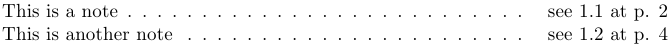
\includegraphics[width=\linewidth-2mm]{img/AlteredAppearenceOfListOfTodos.png}};
% \end{tikzpicture}
% 
% 
% \subsubsection{Tikz externalization issues}
% 
% Using the tikz externalization framework together with todonotes 
% can lead to some problems.
% One solution is to disable the externalization just before the \verb!todo! 
% command is issued and then reactivate externalization afterwards.
% The \verb!ruggedtodo! handles this deactivation and reactivation.
% \begin{verbatim}
% \usetikzlibrary{external}
% \tikzexternalize
% \newcommand{\ruggedtodo}[2][]{\tikzexternaldisable\todo[#1]{#2}\tikzexternalenable}
% \end{verbatim}
% 
% 
% \subsubsection{Highligt text to fix}
% Tobias Winchen provides the following example on how to highlight
% text related to the inserted todonote.
% \makeatletter
% \if@todonotes@disabled
% \newcommand{\hlfix}[2]{#1}
% \else
% \newcommand{\hlfix}[2]{\texthl{#1}\todo{#2}}
% \fi
% \makeatother
% Example \hlfix{wrong text}{fix text}~continues here. 
% Notice that the code relies on the \verb!soul! package.
% \begin{verbatim}
% \makeatletter
% \if@todonotes@disabled
% \newcommand{\hlfix}[2]{#1}
% \else
% \newcommand{\hlfix}[2]{\texthl{#1}\todo{#2}}
% \fi
% \makeatother
% Example \hlfix{wrong text}{fix text}~continues here. 
% \end{verbatim}
% 
% 
% 
% 
%
% \iffalse
% \StopEventually{\PrintChanges\PrintIndex}
% \fi
% \StopEventually{\PrintChanges}
%
% \newpage
% \section{Implementation}
%
% Identifies the package and loads the packages dependences.
%    \begin{macrocode}
\ProvidesPackage{todonotes}[2018/10/17]
\RequirePackage{ifthen}
\RequirePackage{xkeyval}
\RequirePackage{xcolor}
\RequirePackage{tikz}
\usetikzlibrary{positioning}
\usetikzlibrary{shadows}
\RequirePackage{calc}
%    \end{macrocode}
% Implement a function for setting up the todonotes package.
%    \begin{macrocode}
\newcommand\setuptodonotes[1]{\presetkeys{todonotes}{#1}{}}
%    \end{macrocode}
% Some default values are set
%    \begin{macrocode}
\newcommand{\@todonotes@text}{}%
\newcommand{\@todonotes@backgroundcolor}{orange}
\newcommand{\@todonotes@textcolor}{black}
\newcommand{\@todonotes@linecolor}{orange}
\newcommand{\@todonotes@bordercolor}{black}
\newcommand{\@todonotes@tickmarkheight}{0cm}
\newcommand{\@todonotes@textwidth}{\marginparwidth}
\newcommand{\@todonotes@textsize}{\normalsize}
\newcommand{\@todonotes@figwidth}{\linewidth}
\newcommand{\@todonotes@figheight}{4cm}
\newcommand{\@todonotes@figcolor}{black!40}
%    \end{macrocode}
%    \begin{macrocode}
\AtBeginDocument{
\ifx\undefined\phantomsection
\newcommand{\phantomsection}{}
\fi
\ifdim \marginparwidth < 2cm 
\PackageWarning{todonotes}{The length marginparwidth is 
less than 2cm and will most likely cause issues with the 
appearance of inserted todonotes. 
The issue can be solved by adding a line like 
\setlength{\marginparwidth}{2cm} 
prior to loading the todonotes package.} \else\fi%
}
%    \end{macrocode}
%
% \subsection{Declaration of options for the package}
% In this part the various options for
% the package are defined.

% Define the default text strings and set localization options for
% the danish and german languages.
%    \begin{macrocode}
\newcommand{\@todonotes@todolistname}{Todo list}
\newcommand{\@todonotes@MissingFigureText}{Figure}
\newcommand{\@todonotes@MissingFigureUp}{Missing}
\newcommand{\@todonotes@MissingFigureDown}{figure}
\newcommand{\@todonotes@SetTodoListName}[1]
    {\renewcommand{\@todonotes@todolistname}{#1}}
\newcommand{\@todonotes@SetMissingFigureText}[1]
    {\renewcommand{\@todonotes@MissingFigureText}{#1}}
\newcommand{\@todonotes@SetMissingFigureUp}[1]
    {\renewcommand{\@todonotes@MissingFigureUp}{#1}}
\newcommand{\@todonotes@SetMissingFigureDown}[1]
    {\renewcommand{\@todonotes@MissingFigureDown}{#1}}
\newif{\if@todonotes@reverseMissingFigureTriangle}
\DeclareOptionX{catalan}{
    \@todonotes@SetTodoListName{Llista de feines pendents}%
    \@todonotes@SetMissingFigureText{Figura}%
    \@todonotes@SetMissingFigureUp{Figura}%
    \@todonotes@SetMissingFigureDown{pendent}%
}
\DeclareOptionX{croatian}{%
   \@todonotes@SetTodoListName{Popis obveza}%
   \@todonotes@SetMissingFigureText{Slika}%
   \@todonotes@SetMissingFigureUp{Nedostaje}%
   \@todonotes@SetMissingFigureDown{slika}%
}
\DeclareOptionX{danish}{%
    \@todonotes@SetTodoListName{G\o{}rem\aa{}lsliste}%
    \@todonotes@SetMissingFigureText{Figur}%
    \@todonotes@SetMissingFigureUp{Manglende}%
    \@todonotes@SetMissingFigureDown{figur}%
}
\DeclareOptionX{dutch}{%
   \@todonotes@SetTodoListName{Lijst van onafgewerkte taken}%
   \@todonotes@SetMissingFigureText{Figuur}%
   \@todonotes@SetMissingFigureUp{Ontbrekende}%
   \@todonotes@SetMissingFigureDown{figuur}%
}
\DeclareOptionX{english}{%
   \@todonotes@SetTodoListName{Todo list}%
   \@todonotes@SetMissingFigureText{Figure}%
   \@todonotes@SetMissingFigureUp{Missing}%
   \@todonotes@SetMissingFigureDown{figure}%
}
\DeclareOptionX{french}{%
    \@todonotes@SetTodoListName{Liste des points \`a traiter}%
    \@todonotes@SetMissingFigureText{Figure}%
    \@todonotes@SetMissingFigureUp{Figure}%
    \@todonotes@SetMissingFigureDown{manquante}%
    \@todonotes@reverseMissingFigureTrianglefalse
}
\DeclareOptionX{german}{%
    \@todonotes@SetTodoListName{Liste der noch zu erledigenden Punkte}%
    \@todonotes@SetMissingFigureText{Abbildung}%
    \@todonotes@SetMissingFigureUp{Fehlende}%
    \@todonotes@SetMissingFigureDown{Abbildung}%
}
\DeclareOptionX{italian}{
    \@todonotes@SetTodoListName{Elenco delle cose da fare}%
    \@todonotes@SetMissingFigureText{Figura}%
    \@todonotes@SetMissingFigureUp{Figura}%
    \@todonotes@SetMissingFigureDown{mancante}%
}
\DeclareOptionX{ngerman}{%
    \@todonotes@SetTodoListName{Liste der noch zu erledigenden Punkte}%
    \@todonotes@SetMissingFigureText{Abbildung}%
    \@todonotes@SetMissingFigureUp{Fehlende}%
    \@todonotes@SetMissingFigureDown{Abbildung}%
}
\DeclareOptionX{portuguese}{
    \@todonotes@SetTodoListName{Lista de tarefas pendentes}%
    \@todonotes@SetMissingFigureText{Figura}%
    \@todonotes@SetMissingFigureUp{Figura}%
    \@todonotes@SetMissingFigureDown{pendente}%
}
\DeclareOptionX{spanish}{
    \@todonotes@SetTodoListName{Lista de tareas pendientes}%
    \@todonotes@SetMissingFigureText{Figura}%
    \@todonotes@SetMissingFigureUp{Figura}%
    \@todonotes@SetMissingFigureDown{pendiente}%
}
\DeclareOptionX{swedish}{%
    \@todonotes@SetTodoListName{Att g\"{o}ra-lista}%
    \@todonotes@SetMissingFigureText{Figur}%
    \@todonotes@SetMissingFigureUp{Figur}%
    \@todonotes@SetMissingFigureDown{saknas}%
}
%    \end{macrocode}
% Create a counter, for storing the number of inserted todos.
%    \begin{macrocode}
\newcounter{@todonotes@numberoftodonotes}
%    \end{macrocode}
%
% Toggle whether the package should obey the global draft option.
%    \begin{macrocode}
\newif{\if@todonotes@obeyDraft}
\DeclareOptionX{obeyDraft}{\@todonotes@obeyDrafttrue}
\newif{\if@todonotes@isDraft}
\DeclareOptionX{draft}{\@todonotes@isDrafttrue}
\DeclareOptionX{draftcls}{\@todonotes@isDrafttrue}
\DeclareOptionX{draftclsnofoot}{\@todonotes@isDrafttrue}
\newif{\if@todonotes@obeyFinal}
\DeclareOptionX{obeyFinal}{\@todonotes@obeyFinaltrue}
\newif{\if@todonotes@isFinal}
\DeclareOptionX{final}{\@todonotes@isFinaltrue}
%    \end{macrocode}
% Make it possible to disable the functionality
% of the package. If this option is given, the
% commands  |\todo{}| and |\listoftodos| are defined
% as commands with no effect. (But you can still
% compile you document with these commands).
%    \begin{macrocode}
\newif{\if@todonotes@disabled}
\DeclareOptionX{disable}{\@todonotes@disabledtrue}
%    \end{macrocode}
% Show small boxes in the list of todos with the color of the
% inserted todonotes.
%    \begin{macrocode}
\newif{\if@todonotes@colorinlistoftodos}
\DeclareOptionX{colorinlistoftodos}{\@todonotes@colorinlistoftodostrue}
%    \end{macrocode}
% The default style behaves bad when compiled
% with latex (some text placement problems).
% The dvistyle option, changes the visual behavior
% to avoid this text placement problem.
%    \begin{macrocode}
\newif{\if@todonotes@dviStyle}
\DeclareOptionX{dvistyle}{\@todonotes@dviStyletrue}
%    \end{macrocode}
% Create a color option.
%    \begin{macrocode}
\define@key{todonotes.sty}%
    {color}{
        \renewcommand{\@todonotes@backgroundcolor}{#1}
        \renewcommand{\@todonotes@linecolor}{#1}}
%    \end{macrocode}
% Make the background color of the notes as
% an option.
%    \begin{macrocode}
\define@key{todonotes.sty}%
    {backgroundcolor}{\renewcommand{\@todonotes@backgroundcolor}{#1}}
%    \end{macrocode}
% Make the text color of the notes as
% an option.
%    \begin{macrocode}
\define@key{todonotes.sty}%
    {textcolor}{\renewcommand{\@todonotes@textcolor}{#1}}
%    \end{macrocode}
% Make the line color of the notes as
% an option.
%    \begin{macrocode}
\define@key{todonotes.sty}%
    {linecolor}{\renewcommand{\@todonotes@linecolor}{#1}}
%    \end{macrocode}
% Make the color of the notes box color as
% an option.
%    \begin{macrocode}
\define@key{todonotes.sty}%
    {bordercolor}{\renewcommand{\@todonotes@bordercolor}{#1}}
%    \end{macrocode}
% Make the height of the line start marking as
% an option.
%    \begin{macrocode}
\define@key{todonotes.sty}%
    {tickmarkheight}{\renewcommand{\@todonotes@tickmarkheight}{#1}}
%    \end{macrocode}
% Set whether short captions given as arguments to the todo command
% should be included in the inserted todonote.
%    \begin{macrocode}
\newif{\if@todonotes@prependcaptionglobal}
\@todonotes@prependcaptionglobalfalse
\DeclareOptionX{prependcaption}{\@todonotes@prependcaptionglobaltrue}
%    \end{macrocode}
% Make the text width as an option.
%    \begin{macrocode}
\define@key{todonotes.sty}%
    {textwidth}{\renewcommand{\@todonotes@textwidth}{#1}}
%    \end{macrocode}
% Make the text size as an option, accept both |size| and |textsize|. 
%    \begin{macrocode}
\define@key{todonotes.sty}%
    {textsize}{\renewcommand{\@todonotes@textsize}{#1}}
\define@key{todonotes.sty}%
    {size}{\renewcommand{\@todonotes@textsize}{#1}}
%    \end{macrocode}
% Add option for shadows behind the inserted notes
%    \begin{macrocode}
\newcommand{\@todonotes@shadowenabledbydefault}{noshadow}
\DeclareOptionX{shadow}{\renewcommand{\@todonotes@shadowenabledbydefault}{shadow}}
%    \end{macrocode}
% Add option for the default width of the figure inserted with
% |\missingfigure|.
%    \begin{macrocode}
\define@key{todonotes.sty}%
    {figwidth}{\renewcommand{\@todonotes@figwidth}{#1}}
\define@key{todonotes.sty}%
    {figheight}{\renewcommand{\@todonotes@figheight}{#1}}
\define@key{todonotes.sty}%
    {figcolor}{\renewcommand{\@todonotes@figcolor}{#1}}
%    \end{macrocode}
% Make the text width as an option.
%    \begin{macrocode}
% Finally process the given options.
%    \begin{macrocode}
\ProcessOptionsX*
%    \end{macrocode}
% If the |obeyDraft| is given, check whether one of the |draft|, 
% |draftcls| or |draftclsnofoot|
% options are given and enable or disable the functionality of this
% package.
% If the |obeyFinal| option is given together with the |final| option
% the todonotes are disabled.
% The |disable| option will overrule the effect of |obeyDraft|.
%    \begin{macrocode}
\if@todonotes@disabled
\else
	\if@todonotes@obeyDraft
		\@todonotes@disabledtrue
		\if@todonotes@isDraft
			\@todonotes@disabledfalse
		\fi
	\fi
	\if@todonotes@obeyFinal
		\@todonotes@disabledfalse
		\if@todonotes@isFinal
			\@todonotes@disabledtrue
		\fi
	\fi
\fi
%    \end{macrocode}

% \subsection{Options for the todo command}
%
% In this part the various options for 
% commands in the package are defined.
% Set an arbitrarily fill color
%    \begin{macrocode}
\newcommand{\@todonotes@currentlinecolor}{}%
\newcommand{\@todonotes@currentbackgroundcolor}{}%
\newcommand{\@todonotes@currenttextcolor}{}%
\newcommand{\@todonotes@currentbordercolor}{}%
\define@key{todonotes}{color}{%
    \renewcommand{\@todonotes@currentlinecolor}{#1}%
    \renewcommand{\@todonotes@currentbackgroundcolor}{#1}}%
\define@key{todonotes}{linecolor}{%
    \renewcommand{\@todonotes@currentlinecolor}{#1}}%
\define@key{todonotes}{backgroundcolor}{%
    \renewcommand{\@todonotes@currentbackgroundcolor}{#1}}%
\define@key{todonotes}{textcolor}{%
    \renewcommand{\@todonotes@currenttextcolor}{#1}}%
\define@key{todonotes}{bordercolor}{%
    \renewcommand{\@todonotes@currentbordercolor}{#1}}%
%    \end{macrocode}
% Toggle whether there is a shadow behind the inserted notes.
%    \begin{macrocode}
\newif\if@todonotes@useshadow%
\define@key{todonotes}{shadow}[]{\@todonotes@useshadowtrue}%
\define@key{todonotes}{noshadow}[]{\@todonotes@useshadowfalse}%
%    \end{macrocode}
% Define height of the inserted tickmark.
%    \begin{macrocode}
\define@key{todonotes}{tickmarkheight}{%
    \renewcommand{\@todonotes@tickmarkheight}{#1}}%
%    \end{macrocode}
% Set a relative font size
%    \begin{macrocode}
\newcommand{\@todonotes@sizecommand}{}%
\define@key{todonotes}{size}{\renewcommand{\@todonotes@sizecommand}{#1}%
}%
%    \end{macrocode}
% Should the todo item be disabled?
%    \begin{macrocode}
\newif\if@todonotes@localdisable%
\define@key{todonotes}{disable}[]{\@todonotes@localdisabletrue}%
\define@key{todonotes}{nodisable}[]{\@todonotes@localdisablefalse}%
%    \end{macrocode}
% Should the todo item be included in the list of todos?
%    \begin{macrocode}
\newif\if@todonotes@appendtolistoftodos%
\define@key{todonotes}{list}[]{\@todonotes@appendtolistoftodostrue}%
\define@key{todonotes}{nolist}[]{\@todonotes@appendtolistoftodosfalse}%
%    \end{macrocode}
% Should the todo item be displayed inline?
%    \begin{macrocode}
\newif\if@todonotes@inlinenote%
\define@key{todonotes}{inline}[]{\@todonotes@inlinenotetrue}%
\define@key{todonotes}{noinline}[]{\@todonotes@inlinenotefalse}%
%    \end{macrocode}
%    \begin{macrocode}
\newif\if@todonotes@prependcaption%
\define@key{todonotes}{prepend}[]{\@todonotes@prependcaptiontrue}%
\define@key{todonotes}{noprepend}[]{\@todonotes@prependcaptionfalse}%
%    \end{macrocode}
% Should the note in the margin be connected to the insertion point
% in the text?
%    \begin{macrocode}
\newif\if@todonotes@line%
\define@key{todonotes}{line}[]{\@todonotes@linetrue}%
\define@key{todonotes}{noline}[]{\@todonotes@linefalse}%
%    \end{macrocode}
% Should the connection between note and insertion point be drawn
% in a fancy way? (does only work if line=true)
%    \begin{macrocode}
\newif\if@todonotes@fancyline\@todonotes@fancylinefalse%
\define@key{todonotes}{fancyline}[]{\@todonotes@fancylinetrue}%
\define@key{todonotes}{nofancyline}[]{\@todonotes@fancylinefalse}%
%    \end{macrocode}
% Author option.
%    \begin{macrocode}
\newcommand{\@todonotes@author}{}%
\newif\if@todonotes@authorgiven%
\define@key{todonotes}{author}{%
    \renewcommand{\@todonotes@author}{#1}%
    \@todonotes@authorgiventrue}%
\define@key{todonotes}{noauthor}[]{\@todonotes@authorgivenfalse}%
%    \end{macrocode}
% Should the text in the list of todos be different from the text
% in the todonote?
%    \begin{macrocode}
\newcommand{\@todonotes@caption}{}%
\newif\if@todonotes@captiongiven%
\define@key{todonotes}{caption}%
    {\renewcommand{\@todonotes@caption}{#1}%
    \@todonotes@captiongiventrue}%
\define@key{todonotes}{nocaption}[]{\@todonotes@captiongivenfalse}%
%    \end{macrocode}
% Change the current figure width and height.
%    \begin{macrocode}
\newcommand{\@todonotes@currentfigwidth}{\@todonotes@figwidth}
\define@key{todonotes}%
    {figwidth}{\renewcommand{\@todonotes@currentfigwidth}{#1-2pt}}
\newcommand{\@todonotes@currentfigheight}{\@todonotes@figheight}
\define@key{todonotes}%
    {figheight}{\renewcommand{\@todonotes@currentfigheight}{#1-2pt}}
\newcommand{\@todonotes@currentfigcolor}{\@todonotes@figcolor}
\define@key{todonotes}%
    {figcolor}{\renewcommand{\@todonotes@currentfigcolor}{#1}}
%    \end{macrocode}
% Change the width of an inline note.
%    \begin{macrocode}
\newcommand{\@todonotes@inlinewidth}{\linewidth}%
\define@key{todonotes}%
    {inlinewidth}{\renewcommand{\@todonotes@inlinewidth}{#1}}
%    \end{macrocode}
% Change if inline note is written to a separate line or not.
%    \begin{macrocode}
\newif\if@todonotes@inlinepar
\@todonotes@inlinepartrue
\define@key{todonotes}{inlinepar}[]{\@todonotes@inlinepartrue}%
\define@key{todonotes}{noinlinepar}[]{\@todonotes@inlineparfalse}%
%    \end{macrocode}
% Preset values of the options
%    \begin{macrocode}
\presetkeys%
    {todonotes}%
    {linecolor=\@todonotes@linecolor,%
    backgroundcolor=\@todonotes@backgroundcolor,%
    textcolor=\@todonotes@textcolor,%
    bordercolor=\@todonotes@bordercolor,%
    tickmarkheight=0cm,%
    nofancyline,%
    nodisable,%
    noinline,%
    nocaption,%
    noauthor,%
    \@todonotes@shadowenabledbydefault,%
    figwidth=\@todonotes@figwidth,%
    figheight=\@todonotes@figheight,%
    figcolor=\@todonotes@figcolor,%
    line, list,%
    inlinewidth=\linewidth,
    inlinepar}{}%
\@temptokena\expandafter{\@todonotes@textsize}
\edef\next{\noexpand\presetkeys{todonotes}{size=\the\@temptokena}{}}
\next
%    \end{macrocode}
% \subsection{The main code part}
% Here is the actual macros defined.
% If the option "disable" was passed to the package
% define empty commands.
%    \begin{macrocode}
\if@todonotes@disabled%
    \newcommand{\listoftodos}[1][]{}
    \newcommand{\@todo}[2][]{}
    \newcommand{\missingfigure}[2][]{}
\else % \if@todonotes@disabled
%    \end{macrocode}
% Define the |\listoftodos| command and define the 
% appearance of the list of todos.
%    \begin{macrocode}
\newcommand{\listoftodos}[1][\@todonotes@todolistname]
    {\@ifundefined{chapter}{\section*{#1}}{\chapter*{#1}} \@starttoc{tdo}}
\newcommand{\l@todo}
    {\@dottedtocline{1}{0em}{2.3em}}
%    \end{macrocode}
% Define styles used by the todo command
%    \begin{macrocode}
\tikzstyle{notestyleraw} = [
    draw=\@todonotes@currentbordercolor, 
    fill=\@todonotes@currentbackgroundcolor,
    text=\@todonotes@currenttextcolor,
    line width=0.5pt,
    text width = \@todonotes@textwidth - 1.6 ex - 1pt, 
    inner sep = 0.8 ex,
    rounded corners=4pt]
%    \end{macrocode}
%
% \begin{macro}{\@todo}
% Define the |\@todo| command.
%    \begin{macrocode}
\newcommand{\@todo}[2][]{%
%    \end{macrocode}
% Use the global value for determining the default prepend behavior.
%    \begin{macrocode}
\if@todonotes@prependcaptionglobal%
	\@todonotes@prependcaptiontrue%
\else%
	\@todonotes@prependcaptionfalse%
\fi%
%    \end{macrocode}
% Store the original text for later usage and parse the given options.
%    \begin{macrocode}
\renewcommand{\@todonotes@text}{#2}%
\renewcommand{\@todonotes@caption}{#2}%
\setkeys{todonotes}{#1}%
%    \end{macrocode}
%
% Add shadows to the inserted todonotes.
%    \begin{macrocode}
\if@todonotes@useshadow%
\tikzstyle{notestyle} = [notestyleraw,%
    general shadow={shadow xshift=0.5ex, shadow yshift=-0.5ex,%
        opacity=1,fill=black!50}]%
\else%
\tikzstyle{notestyle} = [notestyleraw]%
\fi%
%    \end{macrocode}
% Update notestyles
%    \begin{macrocode}
\tikzstyle{notestyleleft} = [%
    notestyle,%
    left]%
\tikzstyle{connectstyle} = [%
    thick,%
    draw=\@todonotes@currentlinecolor]%
\tikzstyle{inlinenotestyle} = [%
    notestyle,%
    text width=\@todonotes@inlinewidth - 1.6 ex - 1 pt]%
%    \end{macrocode}
% If the option |disable| is given to the command, no output is generated.
%    \begin{macrocode}
\if@todonotes@localdisable%
\else%
%    \end{macrocode}
% Add the item to the list of todos. When the option
% |colorinlistoftodos| is given to the package a small colored 
% square is added in front of the text.
%    \begin{macrocode}
\addtocounter{@todonotes@numberoftodonotes}{1}%
\if@todonotes@appendtolistoftodos%
    \phantomsection%
    \if@todonotes@captiongiven%
    \else%
        \renewcommand{\@todonotes@caption}{#2}%
    \fi%
    \@todonotes@addElementToListOfTodos%
\fi%
%    \end{macrocode}
% Prepend the short caption given if it is requested
%    \begin{macrocode}
\if@todonotes@captiongiven%
    \if@todonotes@prependcaption%
        \renewcommand{\@todonotes@text}{\@todonotes@caption: #2}%
    \fi%
\fi%
%    \end{macrocode}
% Place the todonote as indicated by the options (inline or in a
% marginpar), below is the code for the inline placement.
%    \begin{macrocode}
\if@todonotes@inlinenote%
    \@todonotes@drawInlineNote%
\else%
    \@todonotes@drawMarginNoteWithLine%
\fi%\if@todonotes@inlinenote
\fi%\if@todonotes@localdisable
}%
%    \end{macrocode}
% \end{macro}
% \begin{macro}{drawMarginNoteWithLine}
% Define helper function |drawMarginNoteWithLine|.
%    \begin{macrocode}
\newcommand{\@todonotes@drawMarginNoteWithLine}{%
%    \end{macrocode}
% When the todonote should be placed inside a marginpar, the code
% below is applied.
% First is the current location in the document stored, this enables
% us later to connect this point with the inserted todonote. 
%    \begin{macrocode}
\ifvmode
  \vspace*{-\parskip}%   % backup if we are already in vertical mode
  \vskip-\baselineskip   % (and don't loose that space after a
                         %  pagebreak ...
  \noindent
\fi
\begin{tikzpicture}[remember picture, overlay, baseline=-0.75ex]%
    \node [coordinate] (inText) {};%
\end{tikzpicture}%
\marginpar[{% Draw note in left margin
    \@todonotes@drawMarginNote%
    \@todonotes@drawLineToLeftMargin%
%    \end{macrocode}
% In the book documentclass (which is a twoside layout), the
% |\marginpar| marginpar macro takes two arguments
% |\marginpar[left]{right}|.
% If both arguments are given, latex will decide in which side the
% margin note has to be inserted, and then use the corresponding
% commands.
%    \begin{macrocode}
}]{% Draw note in right margin
    \@todonotes@drawMarginNote%
    \@todonotes@drawLineToRightMargin%
}%
}%
%    \end{macrocode}
% \end{macro}
% \begin{macro}{addElementToListOfTodos}
% Define helper function |addElementToListOfTodos|.
%    \begin{macrocode}
\newcommand{\@todonotes@addElementToListOfTodos}{%
    \if@todonotes@colorinlistoftodos%
        \addcontentsline{tdo}{todo}{%
            \fcolorbox{\@todonotes@currentbordercolor}%
                {\@todonotes@currentbackgroundcolor}%
                {\textcolor{\@todonotes@currentbackgroundcolor}{o}}%
            \ \@todonotes@caption}%
    \else%
        \addcontentsline{tdo}{todo}{\@todonotes@caption}%
    \fi}%
%    \end{macrocode}
% \end{macro}
% \begin{macro}{drawInlineNote}
% Define helper function |useSizeCommand|.
%    \begin{macrocode}
\newcommand{\@todonotes@useSizeCommand}{%
\ifcsname \expandafter\string\@todonotes@sizecommand\endcsname
\csname \expandafter\string\@todonotes@sizecommand\endcsname%
\else
\@todonotes@sizecommand
\fi%
}%
%    \end{macrocode}
% \end{macro}
% \begin{macro}{drawInlineNote}
% Define helper function |drawInlineNote|.
%    \begin{macrocode}
\newcommand{\@todonotes@drawInlineNote}{%
    \if@todonotes@dviStyle%
        {\if@todonotes@inlinepar\par\noindent\fi%
         \begin{tikzpicture}[remember picture]%
            \draw node[inlinenotestyle] {};
         \end{tikzpicture}%
         \if@todonotes@inlinepar\par\fi}%
            \if@todonotes@authorgiven%
                {\noindent \@todonotes@useSizeCommand \@todonotes@author:\,\@todonotes@text}%
            \else%
                {\noindent \@todonotes@useSizeCommand \@todonotes@text}%
            \fi
        {\if@todonotes@inlinepar\par\noindent\fi%
         \begin{tikzpicture}[remember picture]%
            \draw node[inlinenotestyle] {};
         \end{tikzpicture}%
         \if@todonotes@inlinepar\par\fi}%
    \else%
        {\if@todonotes@inlinepar\par\noindent\fi%
         \begin{tikzpicture}[remember picture]%
            \draw node[inlinenotestyle,font=\@todonotes@useSizeCommand]{%
                \if@todonotes@authorgiven%
                    {\noindent \@todonotes@author:\,\@todonotes@text}%
                \else%
                    {\noindent \@todonotes@text}%
                \fi};%
         \end{tikzpicture}%
         \if@todonotes@inlinepar\par\fi}%
    \fi}%
%    \end{macrocode}
% \end{macro}
% \begin{macro}{drawMarginNote}
% Define helper function |drawMarginNote|.
%    \begin{macrocode}
\newcommand{\@todonotes@drawMarginNote}{%
\if@todonotes@dviStyle%
    \begin{tikzpicture}[remember picture]%
        \draw node[notestyle] {};%
    \end{tikzpicture}\\%
    \begin{minipage}{\@todonotes@textwidth}%
    \if@todonotes@authorgiven%
      \@todonotes@useSizeCommand \@todonotes@author \@todonotes@text%
    \else%
      \@todonotes@useSizeCommand \@todonotes@text%
    \fi%
    \end{minipage}\\%
    \begin{tikzpicture}[remember picture]%
        \draw node[notestyle] (inNote) {};%
    \end{tikzpicture}%
\else%
    \let\originalHbadness\hbadness%
    \hbadness 100000%
    \begin{tikzpicture}[remember picture,baseline=(X.base)]%
        \node(X){\vphantom{\@todonotes@useSizeCommand X}};%
        \if@todonotes@authorgiven%
            \draw node[notestyle,font=\@todonotes@useSizeCommand,anchor=north] (inNote) at (X.north)%
                {\@todonotes@author};%
            \node(Y)[below=of X]{};%
            \draw node[notestyle,font=\@todonotes@useSizeCommand,anchor=north] (inNote) at (X.south)%
                {\@todonotes@text};%
        \else%
            \draw node[notestyle,font=\@todonotes@useSizeCommand,anchor=north] (inNote) at (X.north)%
                {\@todonotes@text};%
        \fi%
    \end{tikzpicture}%
    \hbadness \originalHbadness%
\fi}%
%    \end{macrocode}
% \end{macro}
% \begin{macro}{drawLineToRightMargin}
% Define helper function |drawLineToRightMargin|.
%    \begin{macrocode}
\newcommand{\@todonotes@drawLineToRightMargin}{%
\if@todonotes@line%
	\if@todonotes@fancyline%
		\tikz[remember picture,overlay]{%
			\tikzstyle{both}=[line width=3pt, draw, opacity=0.15]%
			\tikzstyle{line}=[shorten >=5pt, line cap=round]%
			\tikzstyle{head}=[shorten >=-1pt, dash pattern=on 0pt off 1pt, ->]%
			\foreach \s in {line,head}{%
				\draw[both,\s]%
					(inNote.north west).. controls +(0:0) and +(90:1.5)..([yshift=1ex] inText);%
			}%
		}%
	\else%
		\begin{tikzpicture}[remember picture, overlay]%
			\draw[connectstyle]%
			([yshift=-0.2cm + \@todonotes@tickmarkheight] inText)%
			-| ([yshift=-0.2cm] inText)%
			-| ([xshift=-0.2cm] inNote.west)%
			-| (inNote.west);%
		\end{tikzpicture}%
	\fi%
\fi}%
%    \end{macrocode}
% \end{macro}
% \begin{macro}{drawLineToLeftMargin}
% Define helper function |drawLineToLeftMargin|.
%    \begin{macrocode}
\newcommand{\@todonotes@drawLineToLeftMargin}{%
\if@todonotes@line%
	\if@todonotes@fancyline%
		\tikz[remember picture,overlay]{%
			\tikzstyle{both}=[line width=3pt, draw, opacity=0.15]%
			\tikzstyle{line}=[shorten >=5pt, line cap=round]%
			\tikzstyle{head}=[shorten >=-1pt, dash pattern=on 0pt off 1pt,->]%
			\foreach \s in {line,head}{%
				\draw[both,\s]%
					(inNote.north east).. controls +(0:0) and +(90:1.5)..([yshift=1ex] inText);%
			}%
		}%
	\else%
		\begin{tikzpicture}[remember picture, overlay]%
			\draw[connectstyle]%
			([yshift=-0.2cm + \@todonotes@tickmarkheight] inText)%
			-| ([yshift=-0.2cm] inText)%
			-| ([xshift=0.2cm] inNote.east)%
			-| (inNote.east);%
		\end{tikzpicture}%
	\fi%
\fi}%
%    \end{macrocode}
% \end{macro}
% \begin{macro}{\missingfigure}
% Defines the |\missingfigure| macro.
%    \begin{macrocode}
\newcommand{\missingfigure}[2][]{%
\setkeys{todonotes}{#1}%
\addcontentsline{tdo}{todo}{\@todonotes@MissingFigureText: #2}%
\par
\noindent
\hfill
\begin{tikzpicture}
\draw[fill=\@todonotes@currentfigcolor, draw = black!40, line width=2pt]
    (-2, -0.5*\@todonotes@currentfigheight-0.5cm)
    rectangle +(\@todonotes@currentfigwidth, \@todonotes@currentfigheight);
\draw (2, -0.5) node[right, text
    width=\@todonotes@currentfigwidth-4.5cm, font=\@todonotes@useSizeCommand] {#2};
\draw[red, fill=white, rounded corners = 5pt, line width=10pt] 
    (30:2cm) -- (150:2cm) -- (270:2cm) -- cycle;
\draw (0, 0.3) node {\@todonotes@MissingFigureUp};
\draw (0, -0.3) node {\@todonotes@MissingFigureDown};
\end{tikzpicture}\hfill
\null\par
}% Ending \missingfigure command
\fi% Ending \@todonotes@ifdisabled
%    \end{macrocode}
% \end{macro}
% \begin{macro}{\todototoc}
% Inserts a reference to the list of todos in the table of contents. If |chapter| is defined, 
% |chapter| is used as level otherwise will |section| be used.
% The |\todototoc| command respects the disable option.
%    \begin{macrocode}
\newcommand{\todototoc}
{%
    \if@todonotes@disabled
    \else
		\addcontentsline{toc}{\@ifundefined{chapter}{section}{chapter}}{\@todonotes@todolistname}%
    \fi
}
%    \end{macrocode}
% \end{macro}
%
% \begin{macro}{\todo}
% Define the |\todo| command as a redirection to |\@todo|.
%    \begin{macrocode}
\newcommand{\todo}[2][]{%
  \if@todonotes@inlinepar
    \ifhmode
      \@bsphack
    \else
      \@savsf\@m
      \@savsk\z@
    \fi
    {\@todo[#1]{#2}}%
    \@esphack%
  \else%
    \@todo[#1]{#2}%
  \fi}
%    \end{macrocode}
% \end{macro}
% \appendix
% \newpage
% \Finale
\endinput

